\chapter{Software architecture}
\label{S:architecture}

% TODO: En este apartado empiezo a poner diagramas, los pongo a color o
% mejor en blanco y negro??
% TODO: a color (no creo que tengamos que imprimir)

“Most systems work better they are kept simple rather than complicated”
\cite{kiss-wiki}. This is the main statement of the KISS principle, acronym for
“Keep it simple, stupid”. KISS philosophy is very used on software development
because code tends to chaos and disorder. If the implementation of a
functionality is not properly thought, it adds complexity to the program work
flow. Therefore, to reduce the architecture entropy should be one of the main
design patterns on any software.

Model-View-Controller (MVC) is a well-known software architecture that consists
on the use of this tree elements to build a user interface. It was introduced 
by Trygve Reenskaug in the seventies \cite{mvc-past-present}. When web
applications appeared, this model was applied in many important projects
like \href{https://support.microsoft.com}{Microsoft Support}. 

% TODO: NO SE COMO PONER UNA WEB COMO EJEMPLO: como cita o hipervinculo??
% TODO: como cita.

\begin{figure}[htb]
	\begin{center}
		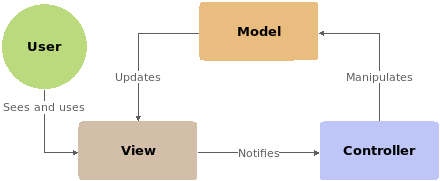
\includegraphics[width=0.5\textwidth]{./figures/mvc.png}
		\caption{Diagram of interactions within the MVC pattern.
				 \cite{mvc-wiki}}
		\label{F:mvc}
	\end{center}
\end{figure}

As shown on Figure \ref{F:mvc}, it is a simple model to represent a user
interface (UI). What user sees is represented by the view. Each time the user 
performs an action, view notifies the controller and it modifies the current
model. Since view is watching changes on the model, this change is detected and,
thus, view is affected.

The problem is that this architecture becomes complex and complex while 
increasing the number of views. Actions from a view can affect other views'
model and this changes can trigger other actions. This complexity could even
generate unexpected loops as Figure \ref{F:mvc-complex} proves.

\begin{figure}[htb]
	\begin{center}
		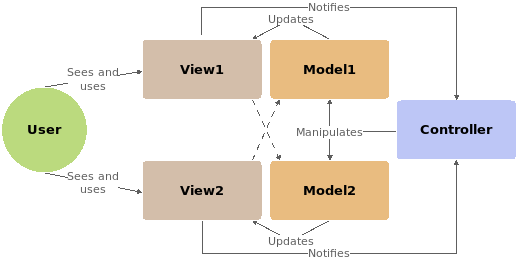
\includegraphics[width=0.6\textwidth]{./figures/mvc-complex.png}
		\caption{Diagram of interactions within the MVC pattern with many views}
		\label{F:mvc-complex}
	\end{center}
\end{figure}

\section{Flux architecture}

In order to solve the MVC scalability problem, Facebook launched Flux, represented
on Figure \ref{F:flux}. Now views are watching a plain object (state) saved
inside the store. Actions are also plain objects that are dispatched changing
the current stored state.

\begin{figure}[htb]
	\begin{center}
		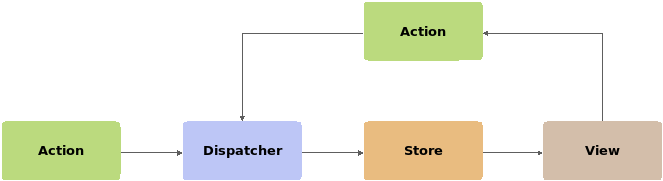
\includegraphics[width=0.7\textwidth]{./figures/flux.png}
		\caption{Diagram of Flux}
		\label{F:flux}
	\end{center}
\end{figure}

Even through views just wait change events produced by the store and render
themselves using the current state information. Note that the render processes
must not call any action.

\section{React}

React is an implementation of the Flux view block. It is a component-based 
JavaScript library to build user interfaces \cite{react-web}. Each React
component can have input properties, state, and must implement a render
function. Moreover, to make things easier, React supports JSX which are
JavaScript files where HTML code can be directly used.

\begin{codefigure}
	\jsxexternal[
		caption=React hello world,
		label=L:react-hello-world,
		%
		classoffset=1,
		morekeywords={HelloMessage, React, Component, ReactDOM},
		classoffset=2,
		morekeywords={<HelloMessage},
	]{source/react-hello-world.jsx}
\end{codefigure}

Listing \ref{L:react-hello-world} shows up an example of React component. It is
stateless, it has a property call name and an easy render function to create a
\textit{div} with text. Render functions can also have components inside
themselves. That way, React creates a component tree \ref{F:react-tree}.

\begin{figure}[htb]
	\begin{center}
		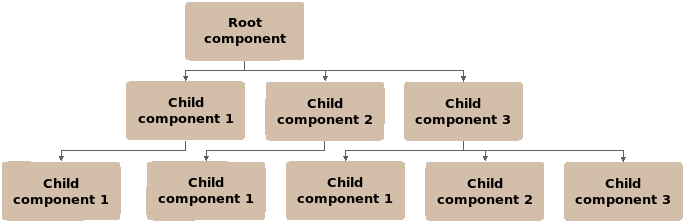
\includegraphics[width=0.7\textwidth]{./figures/react-tree.png}
		\caption{React tree}
		\label{F:react-tree}
	\end{center}
\end{figure}

Components may need to perform actions. Those cannot be performed on render 
function, as seen before. Instead, to do that each component have a lifecyle.
It consists of a set of functions that are triggered when some external events
happen. Most used ones are \textit{"componentWillMount"} and 
\textit{"componentWillUnmount"}. Components also can listen to its view
events, for instance button clicks, to perform actions.

\section{Redux}

Redux was inspired by several important qualities of Flux. Like Flux, Redux
prescribes that the model update logic is concentrated in a certain layer of
the application (“stores” in Flux, “reducers” in Redux) \cite{redux-prior-art}.
Redux have tree principles must be followed \cite{redux-principles}.

\begin{description}
	\item [Single source of truth]
	The state can be stored easily if just one store is used. Furthermore, the
	application will be easy to debug. Once again, keep it simple.
	
	\item [State is read-only]
	The only way to update the state is using actions. Each time the state
	changes, a new independent state must be created.

	\item [Changes are made with pure functions]
	Reducers must be pure functions, that results in the following statement:
	"using the same initial state, repeating the same list of actions must
	produce the same final state".

\end{description}

\begin{figure}[htb]
	\begin{center}
		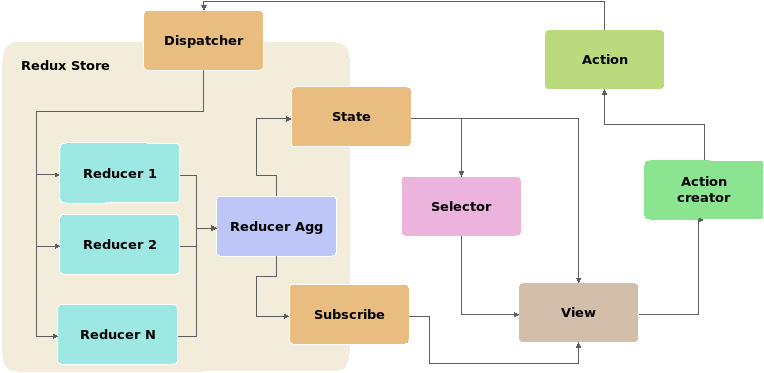
\includegraphics[width=0.8\textwidth]{./figures/redux.png}
		\caption{Redux architecture}
		\label{F:redux-architecture}
	\end{center}
\end{figure}

Figure \ref{F:redux-architecture} shows up the overall Redux's architecture.
First of all, a store must be created. This store contains reducers that map
action, created by action creators, into state changes. If needed, selectors
can be used to cache some state costly transformations. Store also lets 
to subscribe to state change notifications.

\subsection{Action creators}

An action is a plain JavaScript object that contains a field called type to 
identify it and other optional fields. Same type of action can be created in
many places so it is extremely recommended to use action creators.

Action creators are functions that create those objects. Normally are defined
using lambdas. An example of action creator is shown on Listing
\ref{L:redux-action-creator}. This one is intended to create an action that
appends a text item into the state.

\begin{codefigure}
	\jsexternal[
		caption=Redux action creator,
		label=L:redux-action-creator,
	]{source/redux-action-creator.js}
\end{codefigure}

\subsection{Reducers}

Reducers aim to return new states each time an action is produced. They must be
implemented using pure functions. A function must follow tree statements to be 
considered pure.

The fist one is \textbf{mapping}. To fulfill it means that same input always 
results on the same output. Therefore, pure functions can not generate random
numbers, current date, nor depend on external variables. If this statement is
not followed, functions are difficult to test since its return value is
unpredictable. To make a function fulfill mapping is as easy as adding 
unpredictable values as parameters. Listing \ref{L:mapping-example} is an 
example of function that multiplies a random value with a parameter.

\begin{codefigure}
	\jsexternal[
	caption=Mapping example,
	label=L:mapping-example,
	]{source/mapping.js}
\end{codefigure}

The second statement is \textbf{avoid side effects}. This means that functions
must not modify anything outside them. If a pure function needs to access
outside, maybe it is ill-designed. 

\begin{codefigure}
	\jsexternal[
	caption=Avoid side effects example,
	label=L:side-effects-example,
	]{source/no-side-effects.js}
\end{codefigure}

The last one is \textbf{no external mutable}. This means that the output of a
function must be independent to changes other variables. But how can this
happen? Easy, when a JavaScript object is assigned to another variable, it is a
reference of the first one, not a copy. If any of both variables changes, it
will affect also to the other. A simple example of this issue is shown on 
Listing \ref{L:obj-ref}.

\begin{codefigure}
	\jsexternal[
		caption=Object reference effect,
		label=L:obj-ref,
	]{source/obj-ref.js}
\end{codefigure}

Therefore, an example of non pure function due to no external mutation is to
return an object parameter. In order to follow no external mutable principle,
the returned object must be a copy of the one provided as parameter (Figure
\ref{L:no-external-mutation}).

\begin{codefigure}
	\jsexternal[
	caption=No external mutation example,
	label=L:no-external-mutation,
	]{source/no-external-mutation.js}
\end{codefigure}

Then, applying this three principles, Listing \ref{L:redux-reducer} shows up an
example of reducer for the action created on Listing 
\ref{L:redux-action-creator}.

\begin{codefigure}
	\jsexternal[
		caption=Redux reducer,
		label=L:redux-reducer,
	]{source/redux-reducer.js}
\end{codefigure}

This function is called by the store each time an action is dispatched. 
Reducers can be aggregated using a function provided by Redux called
\textit{"combineReducers"}. Listing \ref{L:redux-agg-reducers} shows an example.

\begin{codefigure}
	\jsexternal[
		caption=Reducer aggregation,
		label=L:redux-agg-reducers,
	]{source/redux-agg-reducers.js}
\end{codefigure}

\subsection{Selectors}
\label{S:selectors}

Selectors are functions that can cache the return value and it is just 
recomputed if any of the input parameters changes. For instance, a selector
can be created to select items that starts with letter 'I'. This example is
shown on Listing \ref{L:redux-selector}.

\begin{codefigure}
	\jsexternal[
		caption=Redux selector,
		label=L:redux-selector,
	]{source/redux-selector.js}
\end{codefigure}

\subsection{Store}

Creating a store is as easy as providing the root reducer and the initial state.
Then actions can be dispatched and a function can be subscribed to detect any
state change.

Listing \ref{L:redux-store} shows how to create a store. Selector created in
Section \ref{S:selectors} is used to compute a subset of items just if the
item list has change. Also, several actions are dispatched.

\begin{codefigure}
	\jsexternal[
		caption=Redux store creation and management,
		label=L:redux-store,
	]{source/redux-store.js}
\end{codefigure}

\section{Action observables}

Observables are data streams provided by a library called Reactive Extensions
for JavaScript (rxjs). The idea is to treat those streams as asynchronous 
events and apply fluent query operators to describe behaviors.

\begin{codefigure}
	\jsexternal[
		caption=Rxjs observable to count seconds until last click,
		label=L:rxjs-simple-observable,
	]{source/rxjs-simple-observable.js}
\end{codefigure}

As shown on Listing \ref{L:rxjs-simple-observable}, complex behaviors can be
implemented in an easy to read way using this library. The example shows up
how to count the difference in time between two button clicks. To do that, 
an observable is created to watch the event click of a button. The operator scan
caches the last returned value sending it as first parameter of the callback
function. Last scanned is mapped to get the difference in seconds of last
and current time values. Finally, this difference is printed on a text element.

Since Redux's reducers must be pure functions and there are many complex
behaviors that have to be chained when some actions are produced, Redux
Observables provide a middleware that handles action streams using rxjs
observables. The observable is executed after the action has been reduced.
So Redux architecture (Figure \ref{F:redux-architecture}) must be complemented 
with Figure \ref{F:redux-observables-architecture}.

\begin{figure}[htb]
	\begin{center}
		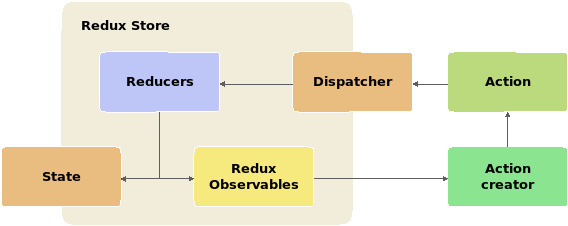
\includegraphics[width=0.6\textwidth]{./figures/redux-observables.png}
		\caption{Redux Observables architecture}
		\label{F:redux-observables-architecture}
	\end{center}
\end{figure}

\section{React-Redux}

To let React and Redux work together, Redux store must be provided to whole
React tree. Also, action creators and state have to be mapped into React
properties.

A package called react-redux adds a React component named \textit{"Provider"}
that inserts a store inside the React tree. Children of \textit{"Provider"} can
connect to it by using the \textit{"connect"} function. It needs two 
parameters, one to map the store state to component's properties and a second 
one to map actions.

\begin{landscape}
\begin{figure}[htp]
	\begin{center}
		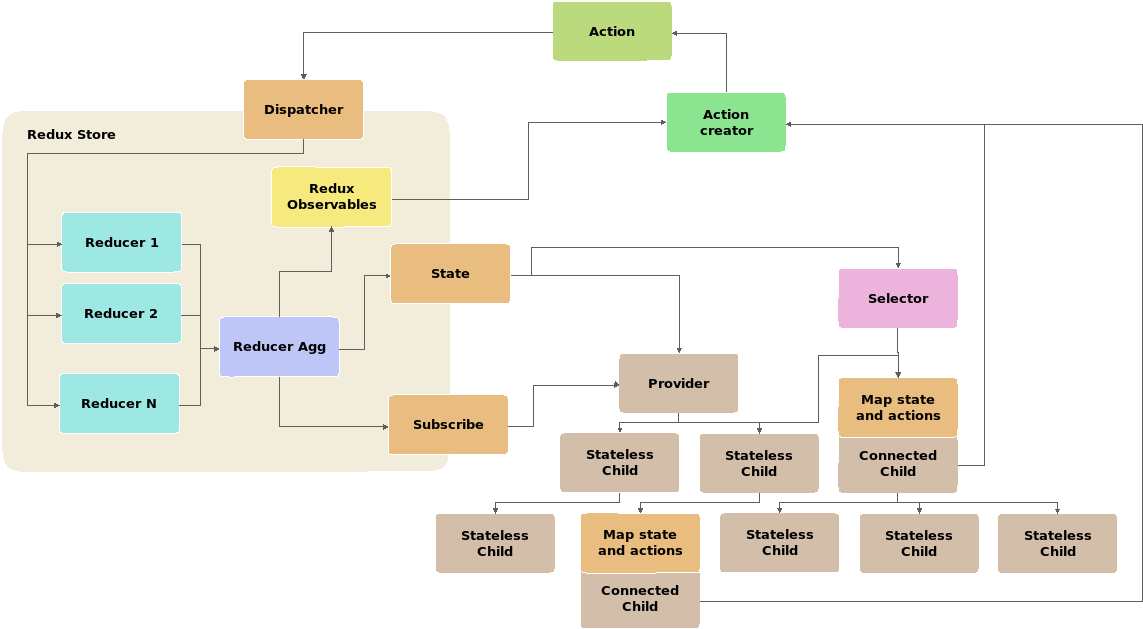
\includegraphics[width=1.3\textwidth]
		{./figures/overall-architecture.png}

		\caption{Overall architecture}
		\label{F:overall-architecture}
	\end{center}
\end{figure}
\end{landscape}





